\documentclass[paper=a4, fontsize=11pt]{scrartcl} % A4 paper and 11pt font size
\usepackage[utf8]{inputenc}
\usepackage{listings}
\usepackage[table,xcdraw]{xcolor}
\usepackage{graphicx}
\usepackage{color}
\usepackage[italian]{babel} % English language/hyphenation
\usepackage{amsmath,amsfonts,amsthm} % Math packages
\usepackage{enumerate}
\usepackage{hyperref}
\usepackage{url}
\usepackage{listings}
\usepackage{color}

\lstset{ 
  basicstyle=\small,        % the size of the fonts that are used for the code
  commentstyle=\color{green},    % comment style
  language=erlang,                 % the language of the code
  numbers=left,                    % where to put the line-numbers; possible values are (none, left, right)
  numbersep=3pt,                   % how far the line-numbers are from the code
  numberstyle=\tiny\color{gray}, % the style that is used for the line-numbers,
  breaklines=true
}

\usepackage{fancyhdr} % Custom headers and footers
\pagestyle{fancyplain} % Makes all pages in the document conform to the custom headers and footers
\fancyhead{} % No page header - if you want one, create it in the same way as the footers below
\fancyfoot[L]{} % Empty left footer
\fancyfoot[C]{} % Empty center footer
\fancyfoot[R]{\thepage} % Page numbering for right footer
\renewcommand{\headrulewidth}{0pt} % Remove header underlines
\renewcommand{\footrulewidth}{0pt} % Remove footer underlines
\setlength{\headheight}{13.6pt} % Customize the height of the header

\numberwithin{equation}{section} % Number equations within sections (i.e. 1.1, 1.2, 2.1, 2.2 instead of 1, 2, 3, 4)
\numberwithin{figure}{section} % Number figures within sections (i.e. 1.1, 1.2, 2.1, 2.2 instead of 1, 2, 3, 4)
\numberwithin{table}{section} % Number tables within sections (i.e. 1.1, 1.2, 2.1, 2.2 instead of 1, 2, 3, 4)

\setlength\parindent{0pt} % Removes all indentation from paragraphs - comment this line for an assignment with lots of text

\graphicspath{{img/}}

%----------------------------------------------------------------------------------------
%	TITLE SECTION
%----------------------------------------------------------------------------------------

\newcommand{\horrule}[1]{\rule{\linewidth}{#1}} % Create horizontal rule command with 1 argument of height

\title{	
\normalfont \normalsize 
\textsc{Sistemi Distribuiti, Università degli studi di Udine} \\ [25pt] % Your university, school and/or department name(s)
\horrule{0.5pt} \\[0.4cm] % Thin top horizontal rule
\huge Distribute a soft real-time 3d multiplayer game\\% The assignment title
\horrule{2pt} \\[0.5cm] % Thick bottom horizontal rule
}

\author{Boubakr Injarn mat. 112194\\Alexandru Pruteanu mat. 111021} % Your name

\date{\normalsize\today} % Today's date or a custom date

\begin{document}

\maketitle % Print the title
\newpage
\tableofcontents
\listoffigures
\newpage
\textbf{\abstractname}

Il seguente progetto consiste nell'implementazione di un gioco in prima persona,
real-time e distribuito. Lo scopo principale è di realizzare l'applicazione tenendo
conto soprattutto di aspetti che riguardano, in particolare, la comunicazione
(cioè affidabilità, consistenza e disponibilità del servizio)

\section{Analisi dei requisiti}
\subsection{Scopo}
Permettere a uno o più utenti di poter comandare una nave spaziale al fine di difendere il pianeta terra dalla minaccia degli asteroidi. Nel secondo caso, ogni utente deve vedere singolarmente le azioni degli altri utenti e lo stato globale del sistema deve essere uguale per tutti.
\subsection{Requisiti}
\begin{enumerate}
\item Il sistema deve dare la massima trasparenza all'utente per quanto riguarda la comunicazione tra i vari moduli. L'utente deve poter avviare l'applicazione (il client) e poter iniziare a giocare la partita.
\item 
\item
\item
\item
\item
\end{enumerate}

\section{Architettura e Design}

In figura \ref{GenArc} è possibile osservare lo schema dell'architettura generale del sistema implementato. Le componenti principali che andremo poi a descrivere sono rappresentate dal client e dal server. Come si osserva, tra questi due vi è un canale full-duplex rappresentato, nel nostro caso, da una connessione \texttt{TCP} (protocollo \texttt{WebSocket}). E' possibile inoltre osservare che i client non comunicano tra di loro in maniera diretta ma attraverso il server master (in figura \ref{Master-Slave} è riportata l'architettura \textit{master-slave} implementata). Master e Slave invece comunicano tra loro al fine di replicare le informazioni (i vari stati di gioco) e garantire una certa disponibilità.

Per permettere la modalità di gioco multiplayer viene utilizzato il protocollo \texttt{WebSocket}, questo perchè il gioco viene eseguito all'interno del browser, il protocollo \texttt{WebSocket}
funziona su \texttt{HTTP} con comunicazione asincrona che possono avvenire concorrente.
Siccome il browser non può ricevere una connessione, ma solo inizializzarla, connessione
fra più client (\texttt{p2p}) non è possibile (attualmente un nuovo protocollo \texttt{WebRTC} si sta
diffondendo per appunto permettere architetture di tipo \texttt{p2p}, purtroppo è una tecnologia ancora troppo giovane).

\begin{figure}
\centering
\includegraphics[width=10cm]{GeneralArchitecture}
\caption{Architettura generale del sistema}
\label{GenArc}
\end{figure}

In figura \ref{GenArc} i client non sono altri che dei browser con supporto per WebGL e WebSocket. All'inizio un client (browser) esegue una richiesta al DNS per ricevere l0indirizzo del WebServer.. Una volta ricevuta la risposta dal DNS con l'indirizzo di uno dei WebServer il client fa una richiesta e riceve tutti gli asset del gioco (js, imagini, css, ...). Il WebServer e solo responsabile per fornire gli asset del gioco, ne di più ne di meno. Infine il client si connete ad uno dei server del gioco (Erlang) e decide di creare una nuova stanza o entrare in una esistente. I server sono scritti nel linguaggio Erlang e con lo scopo primario di essere fault tolerant e distribuiti.

\begin{figure}[h]
\centering
\includegraphics[width=\textwidth]{CAP}
\caption{teorema di Brewer}
\label{CAP}
\end{figure}

In un mondo ideale sarebbe molto bello avere sia Availability che Consistency allo stesso tempo.
In un mondo reale purtroppo cio è impossibile, ed è questo che afferma il teorema di Brewer (CAP Theorem), puoi avere solo 2 cose alla volta (che sono: CP, AP oppure AC), teoriticamente parlando una soluzione AC potrebbe essere possibile, ma purtroppo noi tutti sappiamo che non esiste hardware e reti al mondo che non falliscono mai.
Per il gioco e sistema in analisi sis è optato per un'architettura AP (cioè Availability e Partition tolerance). In un gioco soft realtime è molto più importante un sistema disponibile che consistente (almeno cosi è per questo gioco). In caso di fallimenti è preferibile perdere consistenza (risincronizzare e risolvere conflitti più avanti) e guadagnare disponibilità continua del servizio.

Di seguito vengono elencati i messaggi scambiati fra il client e il server. Per la rappresentazione esterna dei dati viene utilizzato il formato JSON. Lo stesso messaggio ricevuto dal client o dal server può avere funzionalità diverse, ad esempio inizialmente il client manda un messaggio room\_list che server a chiedere al server la lista delle room disponibili, di seguito il server risponde sempre con un messaggio room\_list accompagnato dai dati. Come si può osservare il messaggio è lo stesso ma ha semantica diversa se ricevuto dal client oppure dal server, il tutto e per evitare messaggi duplicati, come add esempio: room\_list\_get, room\_list\_set, ....

Sotto sono elencati i messaggi mandati dal client al server:
\begin{itemize}
\item \texttt{rooms\_list} (richiesta per la lista delle room disponibili)
\item \texttt{room\_join} (richiesta per entrare in una room)
\item \texttt{room\_add} (richiesta per creare una nuova room)
\item \texttt{action\_earth\_collision} (segnalare che c'è stata una collisione con un'asteroide)
\item \texttt{ship\_position} (richiesta della posizione della navicella degli altri giocatori)
\item \texttt{game\_master\_asteroids\_position} (richiesta per la posizione degli asteroidi prima di entrare nel gioco, da un client master)
\item \texttt{game\_ship\_position} (richiesta per la posizione delle navicelle nel gioco)
\item \texttt{action\_ship\_move} (segnalare al server e altri client che la navicella si sta spostando)
\item \texttt{action\_ship\_shot} (segnalare al server e altri client che la navicella ha sparato)
\item \texttt{ping} (messaggio di heartbeat, per dire al server che si è ancora in ascolto e di non chiudere la connessione con il client)
\end{itemize}


Sotto sono elencati i messaggi mandati dal server al client:
\begin{itemize}
\item \texttt{room\_list} (restituisce un elenco delle room disponibili)
\item \texttt{player\_id} (l'identificativo univoco del client)
\item \texttt{room\_players\_number} (numero di giocatori all'interno di una room)
\item \texttt{game\_life} (vita rimasta della terra )
\item \texttt{asteroid\_position} (richiesta per l'invio della posizione degli asteroidi al server)
\item \texttt{asteroid\_position\_set} (messaggio per impostare la nuova posizione degli asteroidi)
\item \texttt{ship\_position\_set} (messaggio per impostare la nuova posizione della navicella spaziale)
\item \texttt{ship\_shoot} (segnala che un altro utente ha sparato)
\item \texttt{servers\_list} (la lista dei server)
\item \texttt{server\_error} (un fallimento nel server)
\item \texttt{game\_reconnect} (risposta affermativa alla richiesta di riconessione al gioco)
\item \texttt{room\_id} (l'identificativo univoco della room)
\item \texttt{pong} (messaggio di heartbeat, risposta al messaggio ping)
\item \texttt{servers\_list\_redirect} (segnala al client la lista aggiornata dei server e di ricontattarne uno)
\item \texttt{remove\_ship\_scene} (messaggio usato per rimuovere una navicella spaziale dalla scena del gioco se un utente si scollega)
\end{itemize}


\subsection{Architettura client}
Per realizzare le funzionalità visuali e interazione del gioco, al client è stata data le precedenti nominate responsabilità, cioè il compito della logica e rendering del gioco che sono sotto controllo di un arbitro che è il server.
L'ambiente scelto per esecuzione del client è all'interno di un browser, la motivazione di una tale scelta sono le varie tecnologie, \texttt{API}, primitive e protocolli
implementati di default che facilitano lo sviluppo e la compatibilità con varie piattaforme.
Per l'implementazione del client sono stati utilizzati i linguaggi di markup \texttt{HTML}e \texttt{CSS} ed il linguaggio di programmazione \texttt{JavaScript}.
Le tecnologie principali utilizzate per la realizzazione del client sono:
\begin{itemize}
\item la libreria \texttt{three.js} \cite{threejs} utilizzata per implementare il rendering del gioco in \texttt{3D};
\item il protocollo \texttt{WebSocket} \cite{websocket} per la comunicazione.
\end{itemize}

Purtroppo un limite imposto dal browser è il modo di comunicazione con gli altri client o server. Le scelte a disposizione sono il classico protocollo \texttt{HTTP}, \texttt{WebSocket} oppure \texttt{WebRTC}. L'ultimo protocollo elencato permette la comunicazione fra i vari client (browser), cioè un'architettura \texttt{P2P}, purtroppo il
protocollo è ancora giovane e non supportato dai vari browser, per questo motivo è stato scelto il protocollo \texttt{WebSocket}. Tale scelta ha influenzato l'architettura
generale del sistema, essendo un protocollo che è basato sul \texttt{HTTP} e non permettendo di aprire una connessione se non richiesta dal browser stesso ha costretto
ad utilizzare dei server che implementano il protocollo \texttt{HTTP} e ha tolto ogni possibile architettura del \texttt{P2P} fra i vari client.


Per una visione più ad alto livello di astrazione, in figura \ref{ClientArc} è possibile osservare l'architettura del singolo client.
Purtroppo non entreremo più in dettaglio per vedere com'è progettato il rendering del client inquanto esula dello scopo del seguente documento, 
ma ci soffermeremo sulla parte di logica e communicazione con il server. Il file e classe responsabile per la communicazione con il server è \texttt{gameClient.js}.
Rimandiamo alla sezione di ? Documentazione Tecnica per una più dettagliata descrizione della communicazione e scambio del messaggi che avviene fra i client e i server.

\begin{figure}
\centering
\includegraphics[width=\textwidth]{ClientArchitecture}
\caption{Architettura del client}
\label{ClientArc}
\end{figure}

\subsection{Erlang}
La scelta del linguaggio per la realizzazione del server è Erlang v.18 \cite{erlang}. Erlang è un linguaggio funzionale, con primitive
per facilitare la communicazione iter-processi/nodi e ampiamente utilizzato per la realizzazione di sistemi distribuiti, real soft-time,
applicazioni non-stop e fault-tolerant.
Tale scelta è sembrata naturale date le funzionalità primitive implementate dal linguaggio e gli scopi della nascita del linguaggio stesso.
Le funzionalità di maggior rilievo che successivamente sono state utilizzate nell'implementazione sono la possibilità di monitorare 
altri processi/nodi ed essere notificati quando muore \cite{erlang-monitor, erlang-supervisor}, librerie per transazioni distribuite \cite{erlang-mnesia} e
un ampio set di librerie (\texttt{OTP}). In particolare il behaviour \texttt{gen\_server} \cite{erlang-gen-server} è risultato
di grande supporto per la realizazzione del server del gioco.


\subsection{Cowboy 2.0}
Come server \texttt{HTTP} è stato deciso di utilizzare la libreria \href{https://github.com/ninenines/cowboy}{Cowboy} interamente scritta in Erlang poiché fornisce un ottimo supporto per le WebSocket (tutte le versioni sia standard che non definitive), modello su cui è basato il progetto.
Uno dei punti di forza di Cowboy sicuramente è la semplicità del codice. I 3 moduli principali che verranno descritti nel dettaglio nella sezione successiva sono di facile comprensione e composti ciascuno da poche righe di codice di base ben documentato, da arricchire, ovviamente, secondo le esigenze del programmatore.

\subsection{Rappresentazione esterna dei dati}

\subsection{Architettura server}
In figura \ref{ServerArc} possiamo invece osservare l'architettura che è stata implementata per il server.

\begin{figure}
\centering
\includegraphics[width=\textwidth]{ServerArchitecture}
\caption{Architettura generale del server}
\label{ServerArc}
\end{figure}

Il server è interamente scritto in Erlang e la libreria principale utilizzata, oltre Cowboy è \href{https://github.com/davisp/jiffy}{Jiffi}. Il progetto è stato diviso in più moduli di cui tre in particolare per la gestione della \textit{websocket}, uno per la gestione delle repliche (o slave) e altri per la gestione della logica di gioco; i moduli vengono di seguito descritti.
\subsubsection{earth\_defender\_app}
Il modulo \texttt{earth\_defender\_app} è responsabile della configurazione e dell'avvio del processo server (nel nostro caso un server Cowboy). Il modulo risponde con la configurazione in \texttt{config.hrl} che contiene il nome dell'host, la porta e un timeout.
Di seguito è possibile osservare la parte di codice dove viene indicato di avviare un server in ascolto sulla porta specificata in fase di creazione della websocket \texttt{>make [...] -port 8888} con protocollo \texttt{http} e inoltrare le richieste al modulo \texttt{websocket\_handler}.
\begin{lstlisting}[basicstyle=\footnotesize]
start(_Type, _Args) ->
  Dispatch = cowboy_router:compile([
    {'_', [{"/websocket/", websocket_handler, []}]}
  ]),
  {ok, _} = cowboy:start_clear(http, 100, [{port, utils:get_port()}], #{
    env => #{dispatch => Dispatch}
  }),
  earth_defender_sup:start_link().
\end{lstlisting}
\subsubsection{earth\_defender\_sup}
\texttt{earth\_defender\_sup} funge da modulo supervisore (\texttt{one for one}), in particolare si occupa di riavviare eventuali singoli processi che terminano/falliscono (vedi figura \ref{Supervisor}).
\begin{figure}
\centering
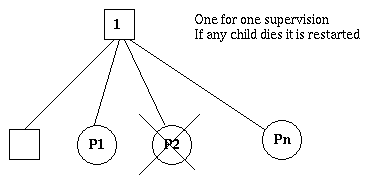
\includegraphics[width=8cm]{sup4}
\caption{Supervisore one for one}
\label{Supervisor}
\end{figure}
\begin{lstlisting}[basicstyle=\footnotesize]
init(_Args) ->
  Procs = [
    {
      local_rooms_state,
      {local_rooms_state, start_link, []},
      permanent,
      infinity,
      worker,
      dynamic
    }
      
  ],
  {ok, {{one_for_one, 10, 10}, Procs}}.
\end{lstlisting}
\subsubsection{websocket\_handler}
\texttt{websocket\_handler} è il modulo principale che si occupa della gestione di tutte le richieste/risposte alla/dalla websocket e da/verso le proprie repliche. Tutte le richieste che arrivano dall'esterno (nel nostro caso dalle operazioni di \texttt{send()} dei vari client) passano per questo modulo attraverso la funzione \texttt{websocket\_handle({text, Msg}, State)} e sono del tipo: \texttt{[evento,dato]} dove \texttt{evento} indica l'azione compiuta dal client (ad esempio per indicare che la nave spaziale si sta spostando) mentre \texttt{dato} contiene gli eventuali dati da trasmettere insieme all'evento (ad esempio la direzione verso la quale la nave si sta spostando), può assumere valore \texttt{null}.
\begin{lstlisting}[basicstyle=\footnotesize][basicstyle=\footnotesize]
websocket_handle({text, Msg}, State) ->
  [Event, Data] = jiffy:decode(Msg),
  case local_rooms_state:is_master() of
    true ->
      case binary_to_list(Event) of
        "game_reconnect" ->
          [Room_id, Player_id, Ship_id] = Data,
          Room_pid = local_rooms_state:get_room_pid(Room_id),
          case Room_id of
            error ->
              reply([<<"server_error">>], State);
            _ ->
              Player_pid = room:get_player_pid(Room_pid, Player_id),
              Player_pid ! {websocket, self()},
              Room_pid ! {player_add, {Player_id, Player_pid, Ship_id}},
              New_state = State#state{player_id = Player_id, room_id = Room_id,
              	 player_pid = Player_pid, room_pid = Room_pid},
              self() ! {servers_list, local_rooms_state:get_servers_list()},
              reply([<<"game_reconnect">>], New_state)
           end;
        "rooms_list" ->
          self() ! {servers_list, local_rooms_state:get_servers_list()},
          reply([<<"rooms_list">>, local_rooms_state:get_rooms_list()], State);
        .
        .
        .
websocket_handle(_Data, State) ->
  {ok, State}.
\end{lstlisting}
In particolare, come si può osservare dal codice sopra, se una istanza di \texttt{Msg} collima con una delle clausole del \texttt{case} allora viene eseguita l'operazione corrispondente altrimenti restituisce un \texttt{Warning}.

%Si noti come per la rappresentazione esterna dei messaggi scambiati tra client e server siano stati utilizzati rispettivamente \href{http://www.json.org/}{\textit{JSON}}

Il presente modulo si occupa anche di rispondere alle richieste inoltrate dai client qualora fosse possibile. La funzione preposta per lo scopo è \texttt{websocket\_info({Event, Data}, State)}.
\begin{lstlisting}[basicstyle=\footnotesize]
websocket_info({Event, Data}, State) ->
  case Event of
    player_id ->
      reply([<<"player_id">>, Data], State);
    room_players_number ->
      reply([<<"room_players_number">>, Data], State);
    .
    .
    .
    Unknown ->
      utils:log("Warning: websocket_info can not handle event:~n~p~n", [Unknown]),
      reply_ok(State)
  end.
\end{lstlisting}
Come nel caso precedente, anche la risposta al client è della forma \texttt{[evento,dato]}. Come varrà descritto successivamente, \texttt{websocket\_info/2} viene invocata da Cowboy ogni qualvolta il modulo riceva un messaggio Erlang.

In caso di fallimento del presente modulo, viene invece invocata la funzione \texttt{terminate/3}, la quale si occupa principalmente, oltre che fornire la causa dell'interruzione, di rimuovere dalla \texttt{room} il player che ha causato il fallimento.
\subsubsection{slave\_handler}
Il presente modulo si occupa, come suggerisce il nome, della gestione delle repliche del server master.

Gli slave (o repliche) possono essere aggiunti in qualsiasi momento dopo l'avvio del master.
Alla prima fase di avvio, queste, contattano il master, il quale si occupa di trasferire l'intero stato del gioco al momento della richiesta (eventuali nuovi aggiornamenti dello stato vengono trasmessi in coda a quest'ultimo messaggio per poi essere successivamente elaborati dalla replica, ottenendo pertanto uno stato consistente).

Dopo la prima fase di sincronizzazione tra il master e lo slave, tutti i messaggi che vengono inoltrati dal client passano poi dal master a tutti gli slaves collegati. E' importante notare che i client contattano sempre solo ed esclusivamente il master pur disponendo degli indirizzi di tutti gli slave (questi ultimi vengono comunicati ad ogni client dal master).

La scelta progettuale fatta in questa fase, potrebbe, giustamente, indurre il lettore a pensare che una soluzione sicuramente più scalabile sarebbe stata quella di suddividere il carico di lavoro del master sulle varie repliche (e quindi, vista l'architettura proposta, tanti master tra loro sincronizzati), tuttavia, trattandosi di un gioco in tempo reale (e vista comunque la non perfetta sincronizzazione di tutti i client) è stato ritenuto opportuno indirizzare tutte le richieste ad una sola "macchina" che funge da master (nel caso specifico anche da arbitro) in modo da permettere a tutti i client di vedere sempre lo stesso stato globale del sistema.



\begin{figure}
\centering
\includegraphics[width=\textwidth]{Master-Slave}
\caption{Architettura Master-Slaves implementata}
\label{Master-Slave}
\end{figure}

In figura \ref{Scaled-Master-Slave} viene proposta una possibile soluzione scalabile di quanto implementato: l'idea consiste nel permettere ad un client, nella prima fase di connessione, di scegliere il server master a cui collegarsi tra quelli eventualmente proposti (si ricorda che deve essere sempre presente almeno un master).

\begin{figure}
\centering
\includegraphics[width=\textwidth]{Scaled_Master-Slave}
\caption{Architettura Masters-Slaves scalare}
\label{Scaled-Master-Slave}
\end{figure}
\subsubsection{Moduli Erlang per la gestione della logica di gioco e lo scambio di messaggi}
I restanti moduli servono principalmente a gestire la logica del gioco e quindi mantenere uno scambio messaggio consistente. Come si può osservare in figura \ref{ServerArc}, lo scambio messaggi avviene solo ed esclusivamente tra i moduli stessi e \texttt{websocket\_handler} (eccezion fatta per \texttt{config}), questi messaggi, come precedentemente affermato, una volta inoltrati al modulo \texttt{websocket\_handler} vengono passati direttamente alla funzione \texttt{websocket\_info/2} per poi, eventualmente, arrivare al client.
\begin{itemize}
\item \texttt{config}: modulo di configurazione iniziale dei parametri del gioco
\item \texttt{local\_rooms\_state}: modulo che contiene lo stato globale del gioco, in particolare la lista di tutte le eventuali \textit{room} attive. Nella sezione successiva verrà descritto dettagliatamente come avvengono le operazioni di creazione e join nella \textit{room}, per ora è sufficiente sapere che ogni player può fare parte di una e una sola \textit{room} e possono esistere più \texttt{room} (almeno una) in modo quindi da permettere il multicast dei messaggi (visto a livello di stato globale) oppure broadcast (visto a livello di singola room).

Il modulo \texttt{websocket\_handler} si occupa di inviare messaggi Erlang al modulo descritto che resta in ascolto con \texttt{handle\_info/2} ed \texttt{handle\_call/3} (in base al tipo di messaggio: sincrono o asincrono) ed in caso di matching esegue le operazioni indicate (si rimanda alla visione del codice per maggiori dettagli).

In generale, il modulo \texttt{local\_rooms\_state} si occupa di creare/eliminare le room di gioco, di aggiungere/rimuovere i player che ne fanno richiesta nella varie room e di smistare i messaggi a queste ultime e/o direttamente ai player, in funzione dell'operazione da eseguire.

\texttt{local\_rooms\_state} si occupa inoltre di tenere sincronizzati il master e gli slave e di definire il nuovo master in caso di fallimento del master originario.


Si può osservare inoltre che tale modulo avvia \texttt{gen\_server}:
\begin{lstlisting}[basicstyle=\footnotesize]
start_link() ->
  gen_server:start_link({local, ?MODULE}, ?MODULE, [], []).
\end{lstlisting}
un generico processo server che fornisce delle funzionalità standard per tracciare e segnalare errori, utile quindi nel caso specifico dove è presente un supervisore che controlla altri nodi.

Nelle prime fasi di implementazione del progetto questo era l'unico modulo ad utilizzare \texttt{gen\_server}, successivamente è stato introdotto in quasi tutti i restanti moduli. 

\item \texttt{room}: modulo che tiene traccia dei player iscritti e dello stato della singola room (posizione navi spaziali, valore della vita, posizione asteroidi, etc\dots).
La funzione \texttt{handle\_info/2} rimane in ascolto di eventuali messaggi ed in generale si occupa di mantenere ed aggiornare lo stato di gioco tra gli iscritti alla room e all'occorrenza inoltrare in broadcast gli aggiornamenti.
\item \texttt{player}: modulo che tiene traccia dell'\texttt{id} del player (oltre ad altre informazioni utili per l'applicazione). Il suo scopo principale è inoltrare eventuali messaggi che giungono dai moduli per la gestione della logica del gioco alla funzione \texttt{websocket\_info} del modulo \texttt{websocket\_handler}.
\end{itemize}

\subsection{Teorema CAP}
In base all'architettura proposta e alle scelte implementative fatte, in figura \ref{CAP} è possibile osservare la posizione del sistema implementato rispetto alle 3 principali garanzie che un sistema distribuito dovrebbe fornire (ricordando che è impossibile fornirle contemporaneamente tutte insieme ma al più due allo stesso tempo).
\begin{figure}
\centering
\includegraphics[width=8cm]{CAP}
\caption{teorema di Brewer}
\label{CAP}
\end{figure}

\begin{itemize}
\item \textit{Coerenza}: il sistema non è perfettamente coerente. A causa di ritardi nell'elaborazione e trasmissione di alcuni messaggi non tutti i nodi (nel nostro caso i client, ma anche i server che replicano i messaggi) vedono esattamente gli stessi dati nello stesso momento e quindi lo stesso stato. Nel caso specifico, è possibile affermare che la coerenza dipende solo ed esclusivamente dal ritardo della rete dato che il modello è di tipo \textit{fat client} e \textit{thin server} ed essendo quindi il server a dover rispondere ai client è poco probabile un ritardo causato dal sovraccarico di quest'ultimo.

Per il progetto proposto, è importante che tutti i client vedano la stessa posizione degli asteroidi, l'esatta posizione delle altre navi spaziali, oltre all'azione che ogni nave sta eseguendo (sparare o muoversi).

Per cercare di mantenere un alto livello di coerenza tenendo conto quindi di possibili ritardi dei messaggi sono state adottate le seguenti strategie:
\begin{itemize}
\item ogni qualvolta un client esegue un operazione di join all'interno della room, quest'ultimo chiede al server la posizione (attuale, al momento della richiesta) di tutti gli asteroidi presenti nella scena del primo client che ha creato la room (o se muore del primo che ha fatto join nella stessa room, il quale avrà già memorizzato la posizione del creatore della room), se anche quest'ultimo muore, del secondo giocatore che ha effettuato un join e via dicendo. Il player al quale viene fatta la richiesta, successivamente, manda in broadcast (anche a se stesso) la posizione attuale di tutti gli asteroidi della propria scena (si noti che in tutto lo scambio messaggi, sicuramente questo è quello più pesante in termini di dimensioni) permettendo quindi a tutti di sincronizzarsi nuovamente sulla stessa scena (ritardo dei messaggi permettendo);
\item un altra strategia che è stata adottata riguarda la posizione delle varie navi all'interno della scena. In particolare, ogni qualvolta un utente decida di spostare la propria nave, quello che sta realmente facendo è comunicare al serve la direzione verso la quale si sta muovendo, il server si occupa successivamente di comunicare a tutti i partecipanti alla room la nuova posizione del player, quest'ultimo compreso, ciò per prevenire la perdita di eventuali messaggi e mantenere sempre coerente la posizione di tutti i player (in sostanza, il server, come più volte affermato, funge da arbitro, "decide" lui la posizione delle navi all'interno della scena);
\item l'ultima strategia riguarda invece la collisione dei vari meteoriti con il pianeta Terra seguito dal relativo aggiornamento del punteggio. A causa del ritardo dei messaggi, non essendoci una perfetta sincronizzazione degli elementi della scena, nel caso specifico gli asteroidi, se in un client, avviene l'azione di collisione poco prima di un altro (assumendo la presenza di soli due giocatori) allora verrebbe tolto il doppio del punteggio (con $n$ giocatori $n*punteggio$), per evitare ciò, il punteggio viene aggiornato solo ed esclusivamente nel momento in cui la collisione avviene nell'ultimo giocatore che è entrato nella room (la scelta è stata casuale, anche scegliendo il primo, il risultato sarebbe stato medesimo). Questa scelta implementativa permane comunque anche in caso di perfetta sincronizzazione degli asteroidi.
\end{itemize}

Per mantenere una buona coerenza, essendo nel caso specifico problematico soprattutto la sincronizzazione dei vari client, avrebbe sicuramente aiutato l'utilizzo di un orologio globale.
\item \textit{Disponibilità}: L'architettura proposta, composta da un master e le relative repliche con, inoltre, la presenza di un modulo supervisore che si occupa di riavviare eventuali processi che muoiono ha reso il sistema in grado di rispondere ad ogni richiesta. Si precisa che più repliche vengono stanziate, maggiore sarà la disponibilità del sistema.
\item \textit{Tolleranza di partizione}: In caso di perdita di messaggi il sistema continua comunque a funzionare ma ciò potrebbe causare una forte incoerenza, un esempio potrebbe essere la mancata comunicazione di collisione da parte dell'ultimo client che ha fatto il join nella room (se si vuole riprendere l'esempio precedente), ciò non impedisce il corretto funzionamento del sistema ma gli altri giocatori che vedono nella propria scena collidere un asteroide senza che il punteggio di aggiorni potrebbero osservare un certo stato di incoerenza.
\end{itemize}

\section{Documentazione tecnica}
Nella seguente sezione si vuole illustrare in maniera più tecnica come avviene la comunicazione tra client e server, alcuni dettagli implementativi e problematiche riscontrate.

La figura \ref{ServerArc} potrebbe trarre in inganno inducendo il lettore a pensare che l'architettura client/server sia di tipo \textit{richiesta/risposta} (comune per server HTTP) ma avendo utilizzato una WebSocket, è possibile sia fare richieste (client $\rightarrow$ server) senza necessariamente attendere una risposta che ricevere risposte (server $\rightarrow$ client) senza necessariamente aver fatto alcuna richiesta, scelta vincente quindi per il tipo di applicazione implementata (si provi a pensare infatti ad un gioco real time con \textit{send/receive} bloccanti).

\subsection{Handshake}
Come già accennato precedentemente, il protocollo di comunicazione utilizzato, appoggiandosi su TCP offre già molte garanzie permettendo di risparmiare un notevole numero di controlli e allo stesso tempo di sfruttare alcune caratteristiche per la gestione di eventuali fallimenti sia da parte dei client che da parte dei server.

La prima fase di comunicazione tra il client ed il server, e quindi la creazione del canale full-duplex tra i due (fase \textit{three way handshake}) avviene sempre nel momento in cui nel client viene selezionata la modalità multiplayer oppure, in caso di fallimento del server, nel qual caso viene creato un nuovo canale (con il server stesso in caso di problema temporaneo di comunicazione oppure con una sua replica).
\subsection{Create room}
Per descrivere come avvengono alcune delle fasi più importanti durante la comunicazione client/server sono stati fatti dei casi d'uso dell'applicazione.

Si tralascia la descrizione del caso "Single player" poiché, come facilmente intuibile, non avviene alcun tipo di comunicazione con il server.

Di seguito si vuole descrivere come avviene la creazione delle room, come illustrato in figura \ref{CreateRoomUC} (il loro scopo è già stato descritto nella sezione precedente), le strutture dati utilizzate, come avviene la comunicazione tra il client ed il server e tra i vari moduli erlang ed il motivo di alcune scelte implementative.

\begin{figure}
\centering
\includegraphics[width=10cm]{MultiplayerCreateRoomUC}
\caption{Create Room in modalità Multiplayer}
\label{CreateRoomUC}
\end{figure}

La creazione della room può essere effettuata da qualsiasi player al completamento delle operazioni di \textit{handshake} con la websocket (ovviamente se non è presente alcuna room iniziale, ovvero \texttt{rooms\_list} restituisce \texttt{[]}, qualcuno ne dovrà creare una).

In figura \ref{CreateRoom} è possibile osservare quali sono le fasi di scambio messaggi che avvengono tra il client ed il server durante la fase di creazione della room.

\begin{figure}
\centering
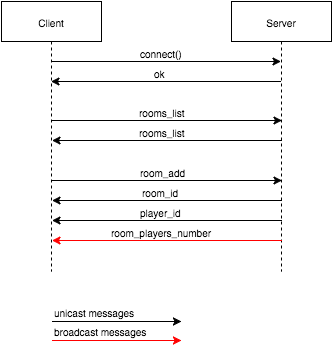
\includegraphics[width=10cm]{MultiplayerCreateRoom}
\caption{Create Room in modalità Multiplayer}
\label{CreateRoom}
\end{figure}


Inizialmente la richiesta parte da \texttt{gameDOMHandler.js}

\begin{lstlisting}[basicstyle=\footnotesize]
document.getElementById('gameRoom-create').addEventListener('click',
				function () {
                    hideComponentGameRoom();
                    gameHandler.server.send('room_add');
                    gameHandler.stop("Loading ...");
                    gameHandler.start();
\end{lstlisting}

L'operazione di \texttt{send()} del client viene inoltrata al modulo erlang \texttt{websocket\_handler} (dando per scontato, ovviamente, che il server sia stato avviato correttamente e la fase di \textit{handshake} sia avvenuta con successo.

\texttt{websocket\_handler} a questo punto avvia la funzione \texttt{websocket\_handle/2} e nello specifico, l'azione trasmessa dal client collima con la clausola:
\begin{lstlisting}[basicstyle=\footnotesize]
"room_add" ->
          Ship_id = Data,
          Room_id = utils:generate_uuid(),
          {_, Room_pid} = room:start_link(Room_id),
          utils:log("Room id:~n~p~n", [Room_id]),
          local_rooms_state:add_room(Room_id, Room_pid),
          Player_id = utils:generate_uuid(),
          Player_pid = player:start(self(), Player_id, Ship_id),
          self() ! {player_id, Player_id},
          Room_pid ! {player_add, {Player_id, Player_pid, Ship_id}},
          New_state = State#state{player_id = Player_id, room_id = Room_id, player_pid =
          	 Player_pid, room_pid = Room_pid, ship_id = Ship_id},
          local_rooms_state:init_broadcast_slaves({binary_to_list(Event), 
          	 {Room_id, Player_id, Ship_id}}),
          reply([<<"room_id">>, Room_id], New_state);
\end{lstlisting}

Come è possibile osservare dal codice sopra, viene assegnato un nome unico identificativo alla room ed inserita nello stato del modulo \texttt{global\_room\_state}, il quale presenta al suo interno un campo di tipo record contenente la lista di tutte le room
\begin{lstlisting}[basicstyle=\footnotesize]
-record(state, {rooms = [], slaves = [], role}).
\end{lstlisting}
La stessa operazione viene eseguita per il player che ha fatto la richiesta ma quest'ultimo viene invece inserito nella lista \texttt{players} del record:
\begin{lstlisting}[basicstyle=\footnotesize]
-record(room_state, {players = [], id, life, asteroids_position, ships_position = [[]]}).
\end{lstlisting}
all'interno della room.

Terminata l'operazione da parte del server, \texttt{websocket\_handler} risponde al client restituendo gli \texttt{id} (da non confondere con il \texttt{PID}) assegnati dal server al player stesso, oltre a comunicare in broadcast il numero di giocatori presenti nella room (che banalmente, in fase di creazione sarà sempre 1).

La scelta di assegnare un nome identificativo unico ad ogni player come ad ogni room nasce dal fatto che, essendo il sistema distribuito (quindi può verificarsi il passaggio di stato da un nodo ad un altro) e ricordando, inoltre, che ad ogni fallimento di un processo erlang il \texttt{PID} cambia, si ha la garanzia che in caso di aggiornamento del \texttt{PID} si leghi il nuovo valore all'id precedentemente definito. 



\subsection{Join room}

\begin{figure}
\centering
\includegraphics[width=10cm]{MultiplayerJoinRoomUC}
\caption{Join Room in modalità Multiplayer}
\label{JoinRoomUC}
\end{figure}

L'operazione di \textit{join} nella room (se ne esiste almeno una, si veda figura \ref{JoinRoomUC}) può essere effettuata da qualsiasi player al completamento della prima operazione di \textit{handshake} con la websocket.

In figura \ref{JoinRoom} è possibile osservare quali sono le fasi di scambio messaggi che avvengono tra il client ed il server nel caso specifico.

\begin{figure}
\centering
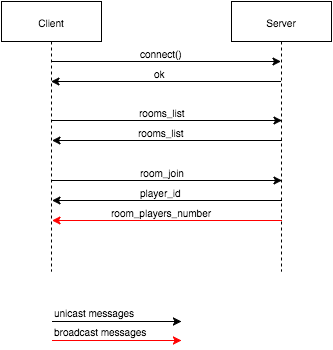
\includegraphics[width=10cm]{MultiplayerJoinRoom}
\caption{Join Room in modalità Multiplayer}
\label{JoinRoom}
\end{figure}

Come nel caso precedente, la richiesta di join parte sempre da \texttt{gameDOMHandler.js} per giungere al modulo erlang \texttt{weboscket\_handler} ed eseguire le opportune azioni.

L'operazione di \textit{join} ha gli stessi effetti dell'operazione di creazione con l'unica differenza che aggiorna semplicemente la lista dei player partecipanti e si occupa di inoltrare nuovamente a tutti la posizione degli asteroidi senza quindi avviare una nuova room. 



\section{Installazione e avvio applicazione}
In questo capitolo vengono date le indicazioni per l'installazione e l'avvio dell'applicazione.
Prima di procedere con l'avvio assicurarsi di avere \texttt{Git}\cite{git} e \texttt{Bower}\cite{bower} installati, nonché di un compilatore e una macchina virtuale per Erlang.
Di seguito vengono elencati i passaggi da seguire per installare sia il client che il server dell'applicazione:
\begin{enumerate}  
\item
Scaricare i file sorgenti del gioco:
\begin{lstlisting}[language=bash]
git clone https://github.com/alexprut/earth-defender.git
\end{lstlisting}

\item
Entrare nella cartella dei file sorgente e cambiare branch:
\begin{lstlisting}[language=bash]
cd earth-defender
git checkout real-time-multiplayer
\end{lstlisting}
\end{enumerate}

Ora che sono stati scaricati i file sorgente del gioco, è possibile procedere con l'installazione del client e server.

\subsection{Client: installazione e configurazione}
\begin{enumerate}  
\item
Entrare nella cartella dei file sorgente del client:
\begin{lstlisting}[language=bash]
cd ./client
\end{lstlisting}

\item
Installare tutte le librerie e dipendenze:
\begin{lstlisting}[language=bash]
bower install
\end{lstlisting}

\item
Configurare il client (si rimanda al file di default in \texttt{./client/js/main.js} dove è incluso una configurazione generale del gioco), di seguito si mostra una possibile configurazione:
\begin{lstlisting}
document.body.onload = function () {
    game = new Game({
        'maxLife': 1000,
        'maxMeteorietes': 200,
        'isMultiplayer': true,
        'maxPlayers': 10,
        'debug': false,
        'servers': ['localhost:8888/websocket', 'localhost:8889/websocket']
    });
    game.init();
};
\end{lstlisting}
\end{enumerate}

Configurato il client è possibile avviare il gioco semplicemente aprendo il file \texttt{./client/index.html}.
Tale passaggio non garantisce però il corretto funzionamento dell'applicazione su tutti i browser senza l'utilizzo di un web server.
Per rendere l'architettura il più realistico possibile si consiglia l' utilizzo di una macchina virtuale sul proprio pc per simulare un web server, in particolare, vista la sua semplicità d'uso
si suggerisce di utilizzare \texttt{Docker}\cite{docker} con eseguire il seguente commando:
\begin{lstlisting}[language=bash]
docker run -p 8000:80 -v "$PWD"/client:/usr/share/nginx/html:ro nginx
\end{lstlisting}
In questo caso specifico è ora sufficiente aprire l'indirizzo \url{http://localhost:8000} dal proprio browser per utilizzare il client del gioco.

\subsection{Server: installazione e configurazione}
\begin{enumerate}
\item
Installare Erlang.mk:
\begin{lstlisting}[language=bash]
curl https://erlang.mk/erlang.mk -o erlang.mk
make -f erlang.mk bootstrap
\end{lstlisting}

\item
I file sorgente del server sono all'interno della cartella \url{./server}:
\begin{lstlisting}[language=bash]
cd ./server
\end{lstlisting}

\item
Configurare il server (si rimanda al file di default in \texttt{./server/src/config.hrl} dove è inclusa la configurazione di default che segue).
\begin{lstlisting}[language=erlang]
-define(EARTH_LIFE, 1000).
-define(EARTH_LIFE_DECREASE, 100).
-define(SHIP_MOVE_FACTOR_X, 2).
-define(SHIP_MOVE_FACTOR_Y, 2).
-define(SHIP_MOVE_FACTOR_Z, 5).
-define(WEBSOCKET_TIMEOUT, 120000).
-define(WEBSOCKET_PORT, 8888).
-define(DEFAULT_HOSTNAME, "localhost").
-define(DEBUG, true).

\end{lstlisting}

\item
Installare tutte le dipendenze ed eseguire il build dell'applicazione:
\begin{lstlisting}[language=bash]
make
\end{lstlisting}
\end{enumerate}
\subsection{Avvio server ed inizio comunicazione}
\begin{enumerate}
\item
Lanciare il server (in maniera veloce) (il server dovrebbe stare in ascolto all'indirizzo \texttt{localhost:8888/websocket} o comunque come indicato nel file di configurazione):
\begin{lstlisting}[language=bash]
make run
\end{lstlisting}
\end{enumerate}

Arrivati a questo punto è possibile collegare client e server.
L'architettura creata è composta da un solo server, il quale funge anche da master. Per aggiungere gli slave (che fungono quindi da repliche) è sufficiente
lanciare il seguente commando:
\begin{lstlisting}[language=bash]
./server/_rel/earth_defender/erts-8.0.2/bin/erl -boot ./server/_rel/earth_defender/releases/1.0.0/earth_defender -sname 'ketchup' -setcookie 'earth_defender' -port 8889 -hostname "localhost" -role slave -master_name earth_defender@host
\end{lstlisting}
Da modificare all'istanziazione di ogni nuovo slave in modo da avviare quest'ultimo su un indirizzo e porta univoci nonché con un nome del nodo univoco, per tale operazione è quindi necessario agire sui seguenti campi \texttt{-sname}, \texttt{-port}, \texttt{-hostname} e \texttt{-master\_name}.

\bibliographystyle{plain}
\bibliography{SD_Injarn_Pruteanu}
\end{document}
